\documentclass[12pt]{article}
\usepackage{hyperref,hyperlatex,url,color,../../chicago,alltt,epsfig,subfigure,pifont}
\setlength{\textwidth}{6.0in}
\setlength{\oddsidemargin}{23pt}
\setlength{\evensidemargin}{23pt}
\setlength{\topmargin}{-0.5in}
\setlength{\textheight}{8.8in}
\newcommand{\libsvm}{$\mbox{\href{http://www.csie.ntu.edu.tw/~cjlin/libsvm}{\sf LIBSVM }}$}
\newcommand{\bsvm}{$\mbox{\href{http://www.csie.ntu.edu.tw/~cjlin/bsvm}{\sf BSVM }}$}

\begin{document}
\setlength{\baselineskip}{18pt}
\begin{center}
{\Large\bf A Practical Guide to Support Vector Classification}

\bigskip

{\bf Chih-Wei Hsu, Chih-Chung Chang, and
 Chih-Jen Lin}\\
\medskip

Department of Computer Science and \\
Information Engineering \\
National Taiwan University \\
Taipei 106, Taiwan (\href{mailto:cjlin@csie.ntu.edu.tw}
{cjlin@csie.ntu.edu.tw})

\end{center}
\medskip

%\maketitle

\begin{abstract}
Support vector machine (SVM) is a popular technique for 
classification. However, beginners who 
are not familiar with SVM often get 
unsatisfactory results since they miss some easy but 
significant steps. In this guide, we propose a 
simple procedure which usually gives reasonable results. 
\end{abstract}

\section{Introduction}
\label{intro}
SVM (Support Vector Machine) is a new technique for data
classification. Even though people consider that it is easier
to use than Neural Networks, however, users who are not 
familiar with SVM often get unsatisfactory results at first.
Here we propose a ``cookbook" approach which usually gives 
reasonable results. 

Note that this guide is not for SVM researchers nor do 
we guarantee the best accuracy. We also do not intend 
to solve challenging or difficult problems. Our purpose 
is to give SVM novices a recipe to obtain acceptable 
results fast and easily.

Although users do not need to understand the underlying 
theory of SVM, nevertheless, we briefly introduce SVM
basics which are necessary for explaining
our procedure. A classification task usually involves 
with training and testing data which 
consist of some data instances. Each instance in the  
training set contains one ``target value" (class labels) 
and several ``attributes" (features). 
The goal of SVM is to produce a model which 
predicts target value of data instances in the testing 
set which are given only the attributes.

Given a training set of
instance-label pairs  $(x_i,y_i), i = 1, \ldots, l$
where $x_i \in R^n$ and $y \in
\{1, -1 \}^l$,
the support vector machines (SVM)
\cite{BB92a,CC95a} require
the solution of the following optimization
problem:
 \begin{eqnarray}
\min_{w,b,\xi} && \frac{1}{2}w^T w + C \sum_{i=1}^l \xi_i
\nonumber \\
\mbox{subject to}&& y_i(w^T \phi(x_i) + b) \geq 1 - \xi_i,\label{svml1}\\
&& \xi_i \geq 0. \nonumber
\end{eqnarray}
Here training vectors $x_i$ are mapped into a
higher (maybe infinite) dimensional space
by the function $\phi$.
Then SVM finds a linear separating hyperplane
with the maximal margin in this
higher dimensional space.
$C>0$ is the penalty parameter of
the error term. Furthermore, $K(x_i, x_j) \equiv 
\phi(x_i)^T\phi(x_j)$ is called the kernel function.
Though new kernels are being proposed by researchers, 
beginners may find in SVM books the following four
basic kernels:
\begin{itemize}
\item linear: $K(x_i, x_j) = x_i ^T x_j$.
\item polynomial: $K(x_i, x_j) = (\gamma {x_i}^T x_j + r)^d$, $\gamma > 0$.
\item radial basis function (RBF): $K(x_i, x_j) = 
\exp(-\gamma{\|x_i-x_j\|}^2)$, $\gamma > 0$.
\item sigmoid: $K(x_i, x_j) = \tanh(\gamma {x_i}^T x_j + r)$.
\end{itemize}
Here, $\gamma$, $r$, and $d$ are kernel parameters.

\subsection{Real-World Examples}

Table \ref{accuracy} presents some real-world examples. These data 
sets are reported from our users who could not obtain reasonable 
accuracy in the beginning. Using the procedure illustrated in this 
guide, we help them to achieve better performance. Details are in 
Appendix \ref{app}. 

\begin{table}
\caption{Problem characteristics and performance comparisons.}
\label{accuracy}
\begin{center}
\begin{tabular}{@{}l|r|r|r|r|r|r@{}}
Applications&\#training&\#testing&\#features&\#classes&Accuracy&Accuracy \\
                &data      &data     &          &       &by users&by our   \\
                &          &         &          &       &        &procedure\\
\hline
Astroparticle\footnotemark[1] & 3,089 & 4,000 & 4 & 2 & 75.2\% & 96.9\% \\
Bioinformatics\footnotemark[2] & 391 & 0\footnotemark[4] & 20 & 3 & 36\% & 85.2\% \\
Vehicle\footnotemark[3] & 1,243 & 41 & 21 & 2 & 4.88\% & 87.8\%
\end{tabular}
\end{center}
\end{table}

\footnotetext[1]{Courtesy of Jan Conrad from Uppsala University, Sweden.}
\footnotetext[2]{Courtesy of Cory Spencer from Simon Fraser University,
Canada \shortcite{JLG03a}.}
\footnotetext[3]{Courtesy of a user from Germany.}
\footnotetext[4]{As there are no testing data, cross-validation instead
of testing accuracy is presented here. Details of cross-validation are 
in Section \ref{cross}.}

These data sets are at \url{http://www.csie.ntu.edu.tw/~cjlin/papers/guide/data/}

\subsection{Proposed Procedure}

Many beginners use the following procedure now:
\begin{itemize}
\item Transform data to the format of an SVM software
\item Randomly try a few kernels and parameters
\item Test
\end{itemize}
We propose that beginners try the following procedure first:
\begin{itemize}
\item Transform data to the format of an SVM software
\item Conduct simple scaling on the data
\item Consider the RBF kernel $K(x,y)=e^{-\gamma\|x-y\|^2}$ 
\item Use cross-validation to find the best parameter
      $C$ and $\gamma$
\item Use the best parameter $C$ and $\gamma$ to train the 
whole training set\footnotemark[5]
\item Test
\end{itemize}
We discuss this procedure in detail in the following 
sections.

\footnotetext[5]{The best parameter might be affected by 
the size of data set but but in practice the one 
obtained from cross-validation is already sutable for the
whole training set.}

\section{Data Preprocessing}

\subsection{Categorical Feature}

SVM requires that each data instance is represented
as a vector of real numbers. Hence, if there are 
categorical attributes, we first have to convert 
them into numeric data. We recommend using $m$ numbers to 
represent an $m$-category attribute. Only one of the $m$
numbers is one, and others are zero. For example,
a three-category attribute such as \{red, green, blue\}
can be represented as (0,0,1),
(0,1,0), and (1,0,0). Our experience indicates that if
the number of values in an attribute is not too many, 
this coding might be more stable 
than using a single number to represent a 
categorical attribute. 

\subsection{Scaling}
\label{scaling}

Scaling them before applying SVM is very important.
\href{ftp://ftp.sas.com/pub/neural/FAQ.html}
{\cite[Part 2 of Neural Networks FAQ]{NN01a}} explains why we scale 
data while using Neural Networks, and most 
of considerations also apply to SVM. 

The main advantage is to avoid attributes in 
greater numeric ranges dominate those in 
smaller numeric ranges. Another advantage is to 
avoid numerical difficulties during the calculation. 
Because kernel values usually depend on the
inner products of feature vectors, e.g. the linear
kernel and the polynomial kernel, large attribute
values might cause numerical problems.
We recommend linearly scaling each attribute to 
the range $[-1,+1]$ or $[0,1]$.

Of course we have to use the same method to 
scale testing data before testing. For example, 
suppose that we scaled the first attribute 
of training data from [-10, +10] to [-1, +1]. 
If the first attribute of testing
data is lying in the range [-11, +8], we must 
scale the testing data to [-1.1, +0.8].

\section{Model Selection}
Though there are only four common kernels 
mentioned in Section \ref{intro}, we must decide 
which one to try first. Then the penalty parameter 
$C$ and kernel parameters are chosen.

\subsection{RBF Kernel}
We suggest that in 
general RBF is a reasonable first choice.
The RBF kernel nonlinearly maps 
samples into a higher dimensional space, so it, 
unlike the linear kernel, can handle the case when
the relation between class labels and 
attributes is nonlinear. Furthermore, the
linear kernel is a special case
of RBF as \cite{SSK02b} shows that the linear kernel 
with a penalty parameter $\tilde{C}$ has the same performance
as the RBF kernel with some parameters $(C, \gamma)$. In
addition, the sigmoid 
kernel behaves like RBF for certain parameters
\cite{HTL03a}.

The second reason is the number of hyperparameters
which influences the complexity of model selection.
The polynomial kernel has more hyperparameters
than the RBF kernel.

Finally, the RBF kernel has less numerical difficulties.
One key point is $0 < K_{ij} \leq 1$ in contrast to 
polynomial kernels of which kernel values may go to 
infinity ($\gamma {x_i}^T x_j + r > 1$) or zero 
($\gamma {x_i}^T x_j + r < 1$) while the degree is large.
Moreover, we must note that the sigmoid kernel is  
not valid (i.e. not the inner product of two vectors) 
under some parameters \cite{VV95a}.

\subsection{Cross-validation and Grid-search}
\label{cross}
There are two parameters 
while using RBF kernels: $C$ and $\gamma$. 
It is not known beforehand which $C$ and 
$\gamma$ are the best for one problem;
consequently some kind of model selection 
(parameter search) must be done. The goal is
to identify good $(C, \gamma)$ so that the classifier 
can accurately predict unknown data (i.e., testing data).
Note that it may not be useful to achieve high 
training accuracy (i.e., classifiers accurately 
predict training data whose class labels are indeed 
known). Therefore, a common way is to separate 
training data to two parts of which one is considered
unknown in training the classifier. Then the prediction
accuracy on this set can more precisely reflect the
performance on classifying unknown data. An improved version of
this procedure is cross-validation.

In $v$-fold cross-validation,
we first divide the training set into $v$ subsets of equal
size. Sequentially one subset is tested using the
classifier trained on the remaining $v-1$ subsets.
Thus, each instance of the whole training set is 
predicted once so the cross-validation accuracy
is the percentage of data which are correctly classified.

The cross-validation procedure can prevent the overfitting
problem. We use Figure \ref{over} which is a binary 
classification problem (triangles and circles) to 
illustrate this issue. Filled circles and triangles 
are the training data while hollow circles
and triangles are the testing data. The testing
accuracy the classifier in Figures \ref{1a} and \ref{1b}
 is not good since it overfits 
the training data. If we think training and testing
data in Figure \ref{1a} and \ref{1b} as the training  and
validation sets in cross-validation, the accuracy is
not good. On the other hand, classifier in \ref{1c} and \ref{1d} without
overfitting training data gives better cross-validation 
as well as testing accuracy. 

\begin{figure}[htbp]
\begin{center}
\begin{tabular}{cc}
\subfigure[Training data and an overfitting classifier]{
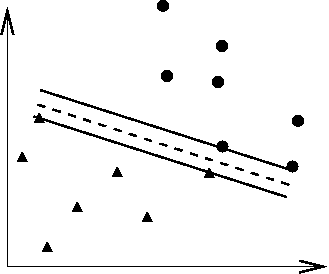
\includegraphics[width=0.48\linewidth]{over1.png}}&
%\epsfig{figure=over1.ps,width=.4\linewidth}}&
\label{1a}
\subfigure[Applying an overfitting classifier on testing data]{
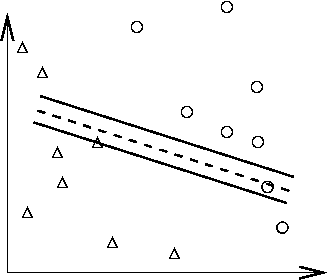
\includegraphics[width=0.48\linewidth]{over2.png}}\\
%\epsfig{figure=over2.ps,width=.4\linewidth}}\\
\label{1b}
\subfigure[Training data and a better classifier]{
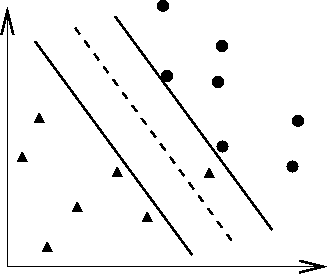
\includegraphics[width=0.48\linewidth]{over3.png}}&
%\epsfig{figure=over3.ps,width=.4\linewidth}}&
\label{1d}
\subfigure[Applying a better classifier on testing data]{
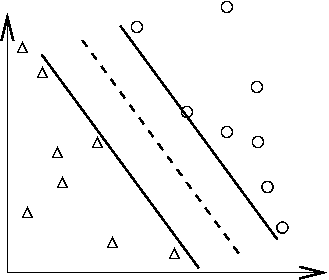
\includegraphics[width=0.48\linewidth]{over4.png}}
%\epsfig{figure=over4.ps,width=.4\linewidth}}
\label{1c}
\end{tabular}
\end{center}
\caption{An overfitting classifier and a better classifier
(\ding{108} and \ding{115}: training data; $\bigcirc$ and $\bigtriangleup$: 
testing data).}
\label{over}
\end{figure}

We recommend a ``grid-search" on $C$ and
$\gamma$ using cross-validation. Basically pairs of $(C,\gamma)$ are tried 
and the one with the best cross-validation accuracy 
is picked. We found that trying
exponentially growing sequences of $C$ and $\gamma$
is a practical method to identify good parameters
(for example, $C=2^{-5},2^{-3},\ldots,2^{15}$, 
$\gamma=2^{-15},2^{-13},\ldots,2^3$).

The grid-search is straightforward but
seems stupid. In fact, there are several 
advanced methods which can save computational 
cost by, for example, approximating the cross-validation 
rate. However, there are two motivations why we prefer the 
simple grid-search approach.

One is that psychologically we may not feel 
safe to use methods which 
avoid doing an exhaustive parameter search 
by approximations or heuristics.
The other reason is that the computational time to find good 
parameters by grid-search is not much more than that 
by advanced methods since there are only 
two parameters.
Furthermore, the grid-search can be easily parallelized 
because each $(C, \gamma)$ is independent.
Many of advanced methods are iterative processes, e.g.
walking along a path, which might be difficult for parallelization. 

\begin{figure}[htbp]
\begin{center}
%\epsfig{figure=coarser.ps,angle=270,width=.45\linewidth,bbllx=70,bblly=325,bburx=465,bbury=625}
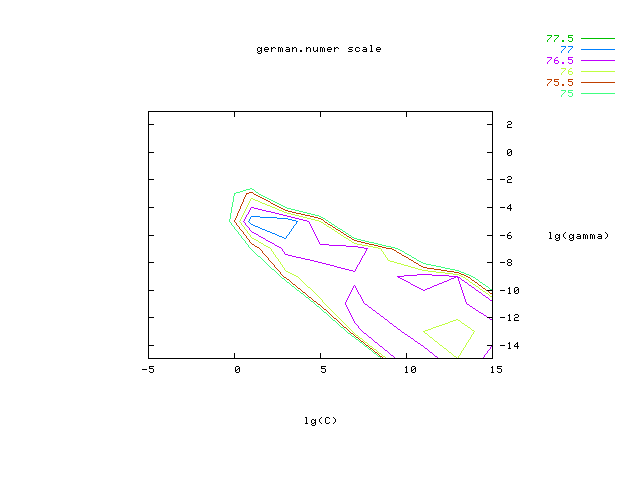
\includegraphics[width=0.75\linewidth,viewport=145 55 625 450,clip]{coarser.png}
%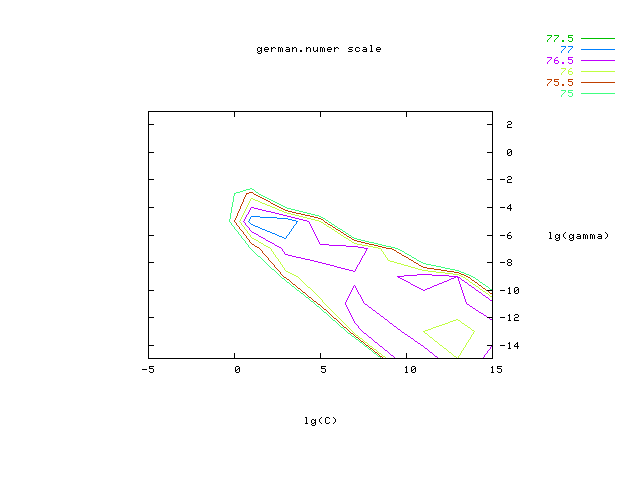
\includegraphics[width=0.9\linewidth]{coarser.pdf}
\end{center}
\caption{Loose grid search on $C=2^{-5},2^{-3},\ldots,2^{15}$ and 
$\gamma=2^{-15},2^{-13},\ldots,2^{3}.$}
\label{coarser}
\end{figure}

\begin{figure}[htbp]
\begin{center}
%\epsfig{figure=finer.ps,angle=270,width=.45\linewidth,bbllx=70,bblly=325,bburx=465,bbury=625}
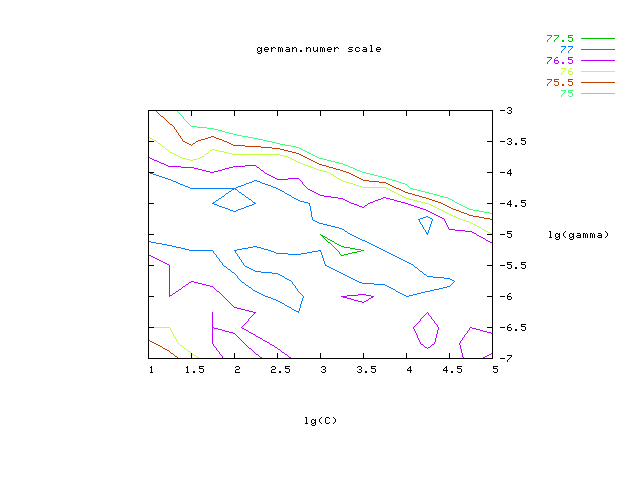
\includegraphics[width=0.75\linewidth,viewport=145 55 625 450,clip]{finer.png}
%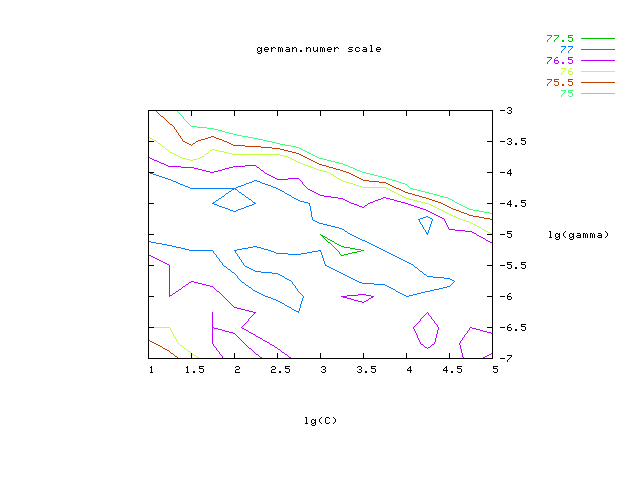
\includegraphics[width=0.9\linewidth]{finer.pdf}
\end{center}
\caption{Fine grid-search on $C=2^{1},2^{1.25},\ldots,2^{5}$ and 
$\gamma=2^{-7},2^{-6.75},\ldots,2^{-3}.$}
\label{finer}
\end{figure}

Since doing a complete grid-search may still be time-consuming, 
we recommend using a coarse grid first. 
After identifying a ``better" region on the
grid, a finer grid search on that region can 
be conducted. To illustrate this, we do an experiment on the problem
\href{http://www.csie.ntu.edu.tw/~cjlin/libsvmtools/binary/german.numer_scale}{{\sf german}} from the 
\href{http://www.ncc.up.pt/liacc/ML/statlog/datasets.html}{Statlog} 
collection \cite{DM94a}. After scaling this set,
we first use a coarse grid (Figure \ref{coarser}) and find that
the best $(C, \gamma)$ is $(2^3, 2^{-5})$ with the cross-validation rate 77.5\%.
Next we conduct a finer grid search on the neighborhood 
of $(2^3, 2^{-5})$ (Figure \ref{finer}) and obtain a better cross-validation 
rate 77.6\% at $(2^{3.25}, 2^{-5.25})$. After the best $(C, \gamma)$ is found, 
the whole training set is trained again
to generate the final classifier.

The above approach works well for problems with 
thousands or more data points. For very large data sets, 
a feasible approach is to randomly choose
a subset of the data set, conduct grid-search on
them, and then do a better-region-only grid-search on
the complete data set.

\section{Discussion}

In some situations, the proposed procedure is not good
enough, so other techniques such as feature selection may
be needed. Such issues are beyond our consideration
here. Our experience indicates that the
procedure works well for data which do not
have many features. 
If there are thousands of
attributes, there may be a need to choose a 
subset of them before giving the data to SVM.

\section*{Acknowledgement}
We thank all users of our SVM software
\libsvm and \bsvm, who help us to identify
possible difficulties encountered by beginners.

\appendix

\section{Examples of the Proposed Procedure}
\label{app}

In this appendix, we compare accuracy
by the proposed procedure with that by general beginners.
Experiments are on the three problems mentioned in
Table \ref{accuracy} by using the software \libsvm
\cite{CC01a}. For each problem, we first list the
accuracy by direct training and testing. Secondly, we show 
the difference in accuracy with and without scaling.
From what has been discussed in Section \ref{scaling},
the range of training set attributes must 
be saved so that we are able to restore them while
scaling the testing set.
Thirdly, the accuracy by the proposed procedure (scaling 
and then model selection) is presented. Finally, we demonstrate 
the use of a tool in \libsvm which does 
the whole procedure automatically.

\begin{itemize}
\item Astroparticle Physics
\begin{itemize}
\item Original sets with default parameters
\begin{alltt}\$./svm-train train.1
\$./svm-predict test.1 train.1.model test.1.predict
 \(\rightarrow\) Accuracy = 66.925%\end{alltt}

\item Scaled sets with default parameters
\begin{alltt}\$./svm-scale -l -1 -u 1 -s range1 train.1 > train.1.scale
\$./svm-scale -r range1 test.1 > test.1.scale
\$./svm-train train.1.scale
\$./svm-predict test.1.scale train.1.scale.model test.1.predict
 \(\rightarrow\) Accuracy = 96.15%\end{alltt}

\item Scaled sets with parameter selection
\begin{alltt}\$python grid.py train.1.scale
\(\cdots\)
2.0 2.0 96.8922\end{alltt}
(Best $C$=2.0, $\gamma$=2.0 with five-fold cross-validation rate=96.8922\%)
\begin{alltt}\$./svm-train -c 2 -g 2 train.1.scale
\$./svm-predict test.1.scale train.1.scale.model test.1.predict
 \(\rightarrow\) Accuracy = 96.875%\end{alltt}

\item Using an automatic script
\begin{alltt}\$python easy.py train.1 test.1
Scaling training data...
Cross validation...
Best c=2.0, g=2.0
Training...
Scaling testing data...
Testing...
Accuracy = 96.875% (3875/4000) (classification)\end{alltt}

\end{itemize}
\item Bioinformatics
\begin{itemize}
\item Original sets with default parameters
\begin{alltt}\$./svm-train -v 5 train.2
 \(\rightarrow\) Cross Validation Accuracy = 56.5217%\end{alltt}

\item Scaled sets with default parameters
\begin{alltt}\$./svm-scale -l 1 -u -1 train.2 > train.2.scale
\$./svm-train -v 5 train.2.scale
 \(\rightarrow\) Cross Validation Accuracy = 78.5166%\end{alltt}

\item Scaled sets with parameter selection
\begin{alltt}\$python grid.py train.2.scale
\(\cdots\)
2.0 0.5 85.1662
 \(\rightarrow\) Cross Validation Accuracy = 85.1662%\end{alltt}
(Best $C$=2.0, $\gamma$=0.5 with five fold cross-validation rate=85.1662\%)

\item Using an automatic script
\begin{alltt}\$python easy.py train.2
Scaling training data...
Cross validation...
Best c=2.0, g=0.5
Training...\end{alltt}

\end{itemize}
\item Vehicle
\begin{itemize}
\item Original sets with default parameters
\begin{alltt}\$./svm-train train.3
\$./svm-predict test.3 train.3.model test.3.predict
 \(\rightarrow\) Accuracy = 2.43902%\end{alltt}

\item Scaled sets with default parameters
\begin{alltt}\$./svm-scale -l 1 -u -1 -s range3 train.3 > train.3.scale
\$./svm-scale -r range3 test.3 > test.3.scale
\$./svm-train train.3.scale
\$./svm-predict test.3.scale train.3.scale.model test.3.predict
 \(\rightarrow\) Accuracy = 12.1951%\end{alltt}

\item Scaled sets with parameter selection
\begin{alltt}\$python grid.py train.3.scale
\(\cdots\)
128.0 0.125 84.8753\end{alltt}
(Best $C$=128.0, $\gamma$=0.125 with five-fold cross-validation rate=84.8753\%)
\begin{alltt}\$./svm-train -c 128 -g 0.125 train.3.scale
\$./svm-predict test.3.scale train.3.scale.model test.3.predict
 \(\rightarrow\) Accuracy = 87.8049%\end{alltt}

\item Using an automatic script
\begin{alltt}\$python easy.py train.3 test.3
Scaling training data...
Cross validation...
Best c=128.0, g=0.125
Training...
Scaling testing data...
Testing...
Accuracy = 87.8049% (36/41) (classification)\end{alltt}

\end{itemize}
\end{itemize}

\bibliographystyle{../../chicago}
\bibliography{../../sdp}
\end{document}

